%%%%%%%%%%%%%%%%%%%%%%%%%%%%%%%%%%%%%%%%%
% baposter Portrait Poster
% LaTeX Template
% Version 1.0 (15/5/13)
%
% Created by:
% Brian Amberg (baposter@brian-amberg.de)
%
% This template has been downloaded from:
% http://www.LaTeXTemplates.com
%
% License:
% CC BY-NC-SA 3.0 (http://creativecommons.org/licenses/by-nc-sa/3.0/)
%
%%%%%%%%%%%%%%%%%%%%%%%%%%%%%%%%%%%%%%%%%
\documentclass[a1paper,portrait,fontscale=0.45]{baposter}

\usepackage[font=small,labelfont=bf]{caption} % Required for specifying captions to tables and figures
\usepackage{booktabs} % Horizontal rules in tables
\usepackage{relsize} % Used for making text smaller in some places
\usepackage{amsmath,amssymb,rotating,placeins,ulem,enumitem,hhline,multirow,diagbox}
\usepackage{sansmath}
\usepackage[scaled]{helvet}
\renewcommand{\familydefault}{\sfdefault} %set default font to sans-serif for entire document.

\sansmath

\graphicspath{{./figures/}} % Directory in which figures are stored

\definecolor{bordercol}{RGB}{255,255,255} % Border color of content boxes
\definecolor{headercol1}{RGB}{255, 102,255} % Background color for the header in the content boxes (left side)
\definecolor{headercol2}{RGB}{153,153,255} % Background color for the header in the content boxes (right side)
\definecolor{headerfontcol}{RGB}{255,255,255} % Text color for the header text in the content boxes
\definecolor{boxcolor}{RGB}{255,255,255} % Background color for the content in the content boxes

% \renewcommand\familydefault{\sfdefault}
\begin{document}

\background{ % Set the background to an image (background.pdf)
  \begin{tikzpicture}[remember picture,overlay]
    \draw (current page.north west)+(-2em,2em) node[anchor=north west]
    % {\includegraphics[height=1.1\textheight]{background}}
    {};
  \end{tikzpicture}
}

% \usepackage{tikz}
% % Bar chart drawing library
% \usepackage{pgfplots}
\usetikzlibrary{shapes,fit}
\tikzset{>=latex}
\usetikzlibrary{shapes.geometric, arrows.meta}

\tikzstyle{host} = [rectangle, rounded corners, minimum width=24mm, minimum height=10mm,text centered, draw=black, fill=red!30,font=\small ]
\tikzstyle{vector} = [rectangle, minimum width=20mm, minimum height=10mm, text centered, draw=black, fill=orange!30,font=\small ]

\tikzstyle{arrow} = [thick,->,>=stealth]
\tikzstyle{arrow2} = [dashed,thick,->,>=stealth]
\tikzstyle{arrow3} = [blue,dotted,thick,<->,>=stealth]
% for patch model

\tikzstyle{hostp} = [rectangle, rounded corners, minimum width=5mm, minimum height=10mm,text centered, draw=black, fill=red!30,font=\small ]
\tikzstyle{vectorp} = [rectangle, minimum width=5mm, minimum height=10mm, text centered, draw=black, fill=orange!30,font=\small ]

\begin{poster}
  {
    columns=3,
    grid=false,
    borderColor=bordercol, % Border color of content boxes
    headerColorOne=headercol1, % Background color for the header in the content boxes (left side)
    headerColorTwo=headercol2, % Background color for the header in the content boxes (right side)
    headerFontColor=headerfontcol, % Text color for the header text in the content boxes
    boxColorOne=boxcolor, % Background color for the content in the content boxes
    headershape=rounded, % Specify the rounded corner in the content box headers
    headerfont=\Large\sf\bf, % Font modifiers for the text in the content box headers
    textborder=rectangle,
    background=user,
    headerborder=open, % Change to closed for a line under the content box headers
    boxshade=plain
  }
  {
    \begin{tabular}{c}
      
\includegraphics[scale=0.12]{logo-imi.jpg}\\
      
\includegraphics[scale=0.23]{logo-ban.png}
    \end{tabular}
  }
  {
    \sf\bf Modelling the effects of mosquito repellent in a two patch system with mobility
  }
  {
    \vspace{.5em} \underline{Kaloian Stoilov}${}^{1,2}$, Peter Rashkov${}^{1}$\\
    {
      \smaller
      ${}^1$ Institute of Mathematics and Informatics, Bulgarian Academy of Sciences,
      ${}^2$ Faculty of Mathematics and Informatics, Sofia University Sveti Kliment Ohridski
      [\texttt{k.stoilov@math.bas.bg}, \texttt{p.rashkov@math.bas.bg}]
    }
  }
  {
    \begin{tabular}{c}
      
\includegraphics[scale=0.07]{logo-fmi.png}\\
      
\includegraphics[scale=0.12]{logo-su.jpg}
    \end{tabular}
  }

  %----------------------------------------------------------------------------------------

  \headerbox{Introduction}{name=introduction,column=0,span=3,row=0}{

    We propose a two patch Ross-Macdonald model with Lagrangian mobility and the use of a repellent, based on the work of [Bichara2016] and [Rashkov2021].
    Each patch is assumed to have separate healthcare capacity.
    We address the question of limiting the infected population sizes for given initial conditions in both patches below the respective capacities at all future times.

    \begin{minipage}{.45\linewidth}
      \centering
      \begin{tikzpicture}[node distance=10mm]
        \node[label={[xshift=-9mm]\small\it humans}] (sh1) [hostp,text width=15mm] {susceptible};

        % right
        \node (ih1) [hostp, right of=sh1, text width=15mm, xshift=10mm] {infected};

        \node (iv1) [vectorp, below of=ih1, yshift=-10mm, text width=15mm] {infected};

        \node[label={[xshift=-5mm] \small\it mosquitos}] (sv1) [vectorp, below of=sh1, yshift= -10mm, text width=15mm] {susceptible};

        \draw [arrow2] (sh1) to (ih1);

        \draw[arrow2] (ih1) to [out=90,in=90] (sh1);

        \draw [arrow] (iv1) to [out=140,in=-50] (sh1) ;

        \draw [arrow] (ih1) to [out=230,in=50] (sv1) ;

        \draw [arrow2] (sv1) -- (iv1);

        \node[label={[label distance=3mm]-90: patch 1 },draw=blue, fit=(sh1)(iv1),inner sep=9mm, rounded corners](FIt1) {};

        % patch 2

        \node[label={[xshift=-7mm]\small\it humans}] (sh2) [hostp,right of=ih1,xshift=30mm,text width=15mm] {susceptible};

        % right
        \node (ih2) [hostp, right of=sh2, text width=15mm, xshift=10mm] {infected};

        \node (iv2) [vectorp, below of=ih2, yshift=-10mm, text width=15mm] {infected};

        \node[label={[xshift=-5mm] \small\it mosquitos}] (sv2) [vectorp, below of=sh2, yshift= -10mm, text width=15mm] {susceptible};

        \draw [arrow2] (sh2) to (ih2);

        \draw[arrow2] (ih2) to [out=90,in=90] (sh2);

        \draw [arrow] (iv2) to [out=140,in=-50] (sh2) ;

        \draw [arrow] (ih2) to [out=230,in=50] (sv2) ;

        \draw [arrow2] (sv2) -- (iv2);

        \node[label={[label distance=3mm]-90: patch 2 },draw=blue, fit=(sh2)(iv2),inner sep=9mm, rounded corners](FIt2) {};

        % arrows between patches
        \draw [arrow3] (sh1) to [out=70,in=110] (sh2) ;
        \draw [arrow3] (ih1) to [out=70,in=110] (ih2) ;
      \end{tikzpicture}
      \captionof{figure}{Model diagram}
    \end{minipage}
    %
    \begin{minipage}{0.55\linewidth}
      \centering
      \begin{tabular}{|c|c|c c|}
        \hline
        Parameter & Definition & patch 1 & patch 2\\
        \hline
        $\beta_{vh}$ & probability of mosquito to human transmission & \multicolumn{2}{c|}{0.5}\\
        $\beta_{hv}$ & probability of human to mosquito transmission & \multicolumn{2}{c|}{0.1}\\
        $a_i$ & human biting rate [day\textsuperscript{-1}] & 0.12 & 0.18 \\
        $M_i$ & female mosquito population & $6 \times 10^7$ & $1.6 \times 10^8$ \\
        $\mu_i$ & rate of mosquito death [day\textsuperscript{-1}] & $\frac{1}{21}$ & $\frac{1}{15}$ \\
        $\tau$ & incubation time in mosquitos [day] & \multicolumn{2}{c|}{10} \\
        $N_i$ & human population & $8 \times 10^6$ & $2 \times 10^7$\\
        $\gamma_i$ & rate of human recovery [day\textsuperscript{-1}] & \multicolumn{2}{c|}{$\frac{1}{14}$}\\
        $p_{ij}$ & mobility of humans from patch i to j & \multicolumn{2}{c|}{varying ($p_{i1}+p_{i2}=1$)}\\
        $\kappa$ & repellent efficiency & \multicolumn{2}{c|}{0.44}\\
        $\bar{u}_i$ & maximum possible repellent coverage & 0.15 & 0.3\\
        $\bar{I}_i$ & maximum healthcare capacity & 0.1 & 0.14\\
        \hline
      \end{tabular}
      \captionof{table}{Table of parameters}
    \end{minipage}

  }

  %----------------------------------------------------------------------------------------

  \headerbox{Model equations}{name=methods,column=0,span=2,below=introduction}{

    \small
    \begin{equation*}
      \begin{split}
        &\dot{X}_1(t) = \beta_{vh} (N_1-X_1(t)) \left(\frac{p_{11} e^{-\mu_1 \tau} a_1 (1-\kappa u_1(t)) Y_1(t)}{p_{11} N_1 + p_{21} N_2} + \frac{p_{12} e^{-\mu_2 \tau} a_2 (1-\kappa u_1(t)) Y_2(t)}{p_{12} N_1 + p_{22} N_2}\right) - \gamma_1 X_1(t) \\
        &\dot{X}_2(t) = \beta_{vh} (N_2-X_2(t)) \left(\frac{p_{21} e^{-\mu_1 \tau} a_1 (1-\kappa u_2(t)) Y_1(t)}{p_{11} N_1 + p_{21} N_2} + \frac{p_{22} e^{-\mu_2 \tau} a_2 (1-\kappa u_2(t)) Y_2(t)}{p_{12} N_1 + p_{22} N_2}\right) - \gamma_2 X_2(t) \\
        &\dot{Y}_1(t) = \beta_{hv} a_1 (M_1-Y_1(t)) \frac{p_{11} (1-\kappa u_1(t)) X_1(t) + p_{21} (1-\kappa u_2(t)) X_2(t)}{p_{11} N_1 + p_{21} N_2} - \mu_1 Y_1(t) \\
        &\dot{Y}_2(t) = \beta_{hv} a_2 (M_2-Y_2(t)) \frac{p_{12} (1-\kappa u_1(t)) X_1(t) + p_{22} (1-\kappa u_2(t)) X_2(t)}{p_{12} N_1 + p_{22} N_2} - \mu_2 Y_2(t) \\
        &u_i(t) \in \mathcal{U}_i = \{u_i:\mathbb{R}_+ \rightarrow [0, \bar{u}_i] \vert u_i \text{- measurable}\}, 0\le \bar u_i<1, i=1,2, \quad U = [0, \bar{u}_1] \times [0, \bar{u}_2], \quad \mathbf{u}(t) = (u_1(t), u_2(t))^T\\
        &\overline{\mathbf{I}} = (\bar{I}_1, \bar{I}_2)^T, \bar{I}_i \in [0, N_i], \quad \mathcal{I} = [0, \bar{I}_1] \times [0, \bar{I}_2] \times [0, M_1] \times [0, M_2]
      \end{split}
    \end{equation*}

  }

  %----------------------------------------------------------------------------------------

  \headerbox{Equilibrium values}{name=equilibrium,column=0,span=2,below=methods}{

    The equilibrium values at maximum repellent coverage can be used to observe cases in which $V(\overline{\mathbf{I}}, \overline{\mathbf{u}})$ is trivial.
    Fixing $u_i (t) \equiv \bar{u}_i, i=1,2$ leads to a cooperative autonomous ODE system for which either the origin is GAS or at most one endemic equilibrium $E^*=(X_1^*, X_2^*, Y_1^*, Y_2^*)^T$ exists, which is GAS.
    If for either patch $X_i^*>\bar{I}_i$, then $X_i(s) > \bar{I}_i$, at some time $s$, implying $V(\overline{\mathbf{I}}, \overline{\mathbf{u}})$ is the origin singleton.
    \begin{center}
      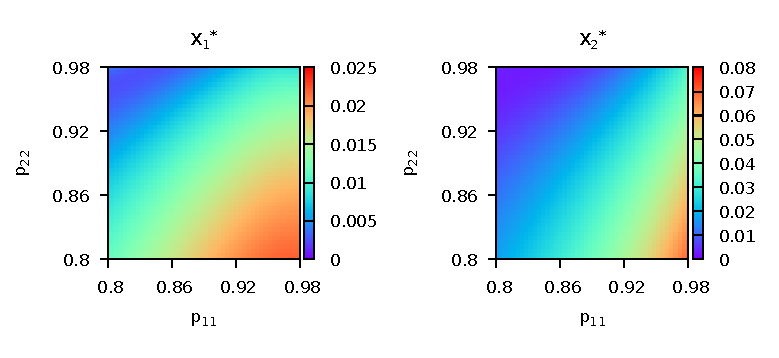
\includegraphics[width=0.7\linewidth]{equilibrium2.pdf}
      \captionof{figure}{Effect of mobility on endemic equilibrium value at maximum repellent coverage ($X_i^*$ as proportion)}
    \end{center}

  }

  %----------------------------------------------------------------------------------------

  \headerbox{Numeric simulations}{name=simulations,column=0,span=2,below=equilibrium}{

    \small
    \centering
    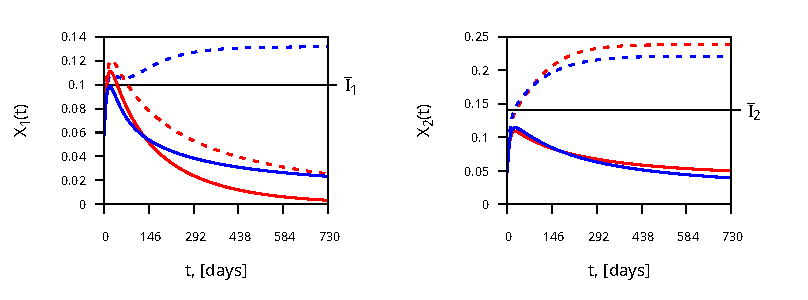
\includegraphics{solution.pdf}
    \captionof{figure}{A plot of $X_i(t)$ as proportion with the initial condition $(0.0572, 0.048, 0.052, 0.044)^T$. Dashed: no repellent used, solid: repellent used ($u_i(t) \equiv \bar u_i$). Red: no mobility between the patches, blue: $p_{11}=p_{22}=0.85$.}

  }

  %----------------------------------------------------------------------------------------

  \headerbox{Viability problem}{name=viability,column=2,below=introduction}{

    The \textbf{viability kernel} $V(\overline{\mathbf{I}}, \overline{\mathbf{u}})$ is the set of initial conditions $(X_1^0, X_2^0, Y_1^0, Y_2^0)^T$, for which a control function $\mathbf{u}(t)$ exists, such that the solutions satisfy

    \begin{equation*}
      X_i(t) \leq \bar{I}_i, i=1,2,\quad  \forall t>0 .
    \end{equation*}

    $V(\overline{\mathbf{I}}, \overline{\mathbf{u}})$ can be characterised as the sub-zero level set of a value function $v$ [Altarovici2013].

    $v$ is the \textbf{viscosity solution} of the HJB equation
    \begin{equation*}
      \min\left\{\lambda v(\mathbf{z}) + \mathcal{H}(\mathbf{z}, \nabla{v}), v(\mathbf{z}) - \Gamma(\mathbf{z})\right\} = 0, \quad \mathbf{z} \in \mathbb{R}^4
    \end{equation*}
    \begin{equation*}
      \mathcal{H}(\mathbf{z}, \nabla{v}) = \max_{\mathbf{u} \in U} \langle -\mathbf{F}(\mathbf{z}, \mathbf{u})\nabla{v}\rangle, ~\mathbf{F} - \text{RHS}
    \end{equation*}
    \begin{equation*}
      \Gamma(\mathbf{z}) =
      \begin{cases}
        \min\limits_{\mathbf{z}' \in \mathcal{I}} |\mathbf{z}-\mathbf{z}'|, \quad \mathbf{z} \in \Omega \setminus \mathcal{I} \\
        -\min\limits_{\mathbf{z}' \in \Omega \setminus \mathcal{I}} |\mathbf{z}-\mathbf{z}'|, \quad \mathbf{z} \in \mathcal{I}
      \end{cases}
    \end{equation*}
    The HJB equation can be numerically integrated using WENO methods [Osher2003].

  }

  %----------------------------------------------------------------------------------------

  \headerbox{Mobility and the viability kernel}{name=mobility,column=2,below=viability}{

    To measure the effects of mobility on the viability kernel $V(\overline{\mathbf{I}}, \overline{\mathbf{u}})$, the volume of its numeric approximation can be compared for various mobilities.
    The case of independent patches, i.e. $p_{11}=p_{22}=1$ can be used as a reference metric. \\

    \centering
    \begin{tabular}{ | c| c c c c|}
      \hline
      \backslashbox{$p_{22}$}{$p_{11}$}& 0.8 & 0.85 & 0.9 & 0.95 \\
      \hline
      0.95 & 3.427 & 3.447 & 3.467 & 3.486\\
      0.9 & 3.468 & 3.487 & 3.507 & 3.527\\
      0.85 & 3.498 & 3.517 & 3.536 & 3.554\\
      0.8 & 3.519 & 3.540 & 3.559 & 3.580\\
      \hline
    \end{tabular}
    \captionof{table}{Viability kernel volume (relative to no mobility)}

  }

  %----------------------------------------------------------------------------------------

  \headerbox{References}{name=references,column=2,span=1,below=mobility}{

    \small
    \begin{itemize}
      \item A. Altarovici, O. Bokanowski, H. Zidani. A general Hamilton-Jacobi framework for non-linear state-constrained control problems. \textit{ESAIM Control. Optim. Calc. Var.} 19:337-357, 2013
      \item D. Bichara, C. Castillo-Chavez, Vector-borne diseases models with residence times - A Lagrangian perspective, \textit{Math. Biosci.}, 281:128-138, 2016
      \item S. Osher, R. Fedkiw. \textit{Level Set Methods and Dynamic Implicit Surfaces}, Springer, 2003
      \item P. Rashkov, A model for a vector-borne disease with control based on mosquito repellents: A viability analysis, \textit{J. Math. Anal. Appl.}, 498:124958, 2021
    \end{itemize}

  }

\end{poster}
\end{document}
